\documentclass[conference]{IEEEtran}
\usepackage{cite}
\usepackage{amsmath,amssymb,amsfonts}
\usepackage{algorithmic}
\usepackage{graphicx}
\usepackage{textcomp}
\usepackage{xcolor}
\usepackage{float}
\usepackage{booktabs}
\usepackage{url}
\usepackage{siunitx}

\def\BibTeX{{\rm B\kern-.05em{\sc i\kern-.025em b}\kern-.08em
    T\kern-.1667em\lower.7ex\hbox{E}\kern-.125emX}}

\begin{document}

\title{ML441 Assignment 3}

\author{\IEEEauthorblockN{RH Buhr, 26440873}
\IEEEauthorblockA{\textit{BDatSci Programme, 4th Year} \\
\textit{Stellenbosch University}\\
Stellenbosch, South Africa \\
26440873@sun.ac.za}
}

\maketitle

\begin{abstract}

\end{abstract}

\section{\textbf{Introduction}}

\section{\textbf{Background}}

\subsection{\textbf{Recurrent Neural Networks}}

Recurrent Neural Neworks are a type of neural network specifically designed to handle sequential data, where there exists temporal dependencies between observations. RNNs incorporate feedback connections that allow information from prior steps to influence future predictions, which is what makes them well-suited for time series data, such as language translation, natural language processing, sentiment analysis, speech recognition, image captioning, etc.

RNNs extend traditional neural networks by incorporating a hidden state that carries information from one time step to the next. This creates a feedback loop, allowing the network to retain context from previous time steps and use it to influence the current time step. At each time step, the RNN processes the new input together with the hidden state from the previous time step, which allows the model to capture temporal dependencies in time series data. Unlike traditional neural networks, like feedforward neural networks, RNNs share hyperparameters across time steps and are trained using backpropagation through time, as opposed to regular backpropagation \cite{ibm_rnn}.

\begin{figure}[H]
  \centering
  \includegraphics[width=0.65\linewidth]{images/ibm_rnn.jpg}
  \caption{Rolled and unrolled views of an RNN (\cite{ibm_rnn}).}
  \label{fig:ibm_rnn}
\end{figure}

Figure~\ref{fig:ibm_rnn} shows a rolled RNN with its unrolled counterpart which has been unrolled over time. Each time step takes $X_t$ and the previous hidden state as input, produces and output $Y_t$ and passes the hidden state to the next time step.

\subsubsection{\textbf{Elman RNN}}

The Elman RNN is considered the vanilla RNN. Its defining factor is the hidden state that stores information from the previous time steps and passes it along to the next time step.

Formally, the Elman RNN is defined as:

$$
h_t = \sigma_h(W_x x_t + W_h h_{t-1} + b_h)
$$

$$
y_t = \sigma_y(W_y h_t + b_y)
$$

where:

\begin{itemize}
    \item $x_t$ is the input vector at time step t.
    \item $y_t$ is the output vector at time step t.
    \item $h_t$ is the hidden state at time step t.
    \item $W_x$ is the input weight matrix.
    \item $W_h$ is the recurrent weight matrix.
    \item $W_y$ is the output weight matrix.
    \item $b_h$ is the hidden state bias term.
    \item $b_y$ is the output bias term.
    \item $\sigma_h$ is a non-linear activation function (e.g. ReLu, sigmoid, tanh).
    \item $\sigma_y$ is an activation function suited for the machine learning task at hand (e.g. softmax for multi-class classification).
\end{itemize}

The inclusion of $W_h h_{t-1}$ in the hidden state of Elman RNNs distinguishes them from traditional models and allows them to maintain memory of past context \cite{elman_rnn}.

\subsubsection{\textbf{Jordan RNN}}

Unlike the Elman RNN, where the hidden state depends on the previous hidden states, the Jordan RNN hidden state depends on previous outputs. This allows the Jordan RNN to integrate information from its own past predictions when updating the current hidden layer.

Formally, the Jordan RNN is defined as:

$$
h_t = \sigma_h(W_x x_t + W_h y_{t-1} + b_h)
$$

$$
y_t = \sigma_y(W_y h_t + b_y)
$$

The use of $W_h y_{t-1}$ in the hidden state instead of $W_h h_{t-1}$ is what sets Jordan RNNs apart from Elman RNNs. This means Jordan RNNs capture sequential information differently than Elman RNNs, which can make them more efficient in settings where the model's own predictions strongly influence the outcome of the current and future time steps \cite{jordan_rnn}.

\subsubsection{\textbf{Multi-RNN}}

Multi-RNNs can be thought of as a combination between Elman and Jordan RNNs by incorporating feedback from both the previous hidden state and the previous output. This allows Multi-RNNs to model sequential information more flexibly, since the current hidden representation does not only depend on the internal memory of the network but also its previous predictions.

The Multi-RNN can be expressed as:

$$
h_t = \sigma_h(W_x x_t + W_{hh} y_{t-1} + W_{hy} y_{t-1} + b_h)
$$

$$
y_t = \sigma_y(W_y h_t + b_y)
$$

The difference is captured in the inclusion of $W_{hh} y_{t-1} + W_{hy} y_{t-1}$ in the hidden state allowing Multi-RNNs to capture richer temporal information.

\subsubsection{\textbf{RNN Limitations}}

While RNNs are powerful tools for time series problems, they suffer from critical limitations, especially when faced with long sequences. The main issue under consideration is known as the Vanishing/Exploding Gradient Problem. During backpropagation through time, gradients can either shrink to near zero or grow excessively. This makes it difficult for the network to capture long-term dependencies and can lead to unstable learning. As a result, RNNs often struggle when context from distant time steps is needed to accurately predict the current time step. Mitigations include, gradient clipping, selection of problem appropriate activation functions, better weight initialization, learning rate control, and the use of more advanced architectures like LSTM \cite{rnn_problems}. 
\subsection{\textbf{Datasets}}

The recurrent neural networks were trained and evaluated across five distinct datasets to provide a comprehensive assessment of their performance across diverse tasks.

\subsubsection{\textbf{AMD Stock Data}}

The AMD dataset records AMD (Advanced Micro Devices) stock data over a period of 40 years. The dataset records 10098 instances of 7 variables:

\begin{itemize}
    \item \texttt{Date}: Date the instance was recorded in the format 'yyyy-mm-dd'.
    \item \texttt{Open}: The price at which the stock first traded on the trading day.
    \item \texttt{High}: The highest price the stock reached during the trading day.
    \item \texttt{Low}: The lowest price the stock reached during the trading day.
    \item \texttt{Close}: The final price of the stock when the market closed on that day.
    \item \texttt{Adj Close}: The closing price adjusted for corporate actions like stock splits or dividends.
    \item \texttt{Volume}: The total number of shares traded on that day.
\end{itemize}

This is a regression problem, with \texttt{Adj Close} as the response, instead of \texttt{Close}, because it reflects the true economic value of the stock by incorporating adjustments, these adjustments ensure the data more accurately reflects the stock market trends.

\begin{figure}[H]
    \centering
    \includegraphics[width=0.5\textwidth]{images/amd_adj_close.pdf}
    \caption{AMD Adjusted Closing Prices Over Time}
    \label{fig:amd_adj_close}
\end{figure}

Figure~\ref{fig:amd_adj_close} displays how AMD's adjusted closing price fluctuated from 1980 through 2020. The series is clearly non-stationary, with periods of sharp growth and declines. The overall trend is upward, even though there are multiple crashes. Most notably around the early 2000s dot-com bubble and the 2008 financial crisis. The defining upward trend, showing rapid growth, started in 2020.

To formally asses stationarity, and Augmented Dickey-Fuller (ADF) test was conducted. The ADF test is a widely used statistical procedure for detecting unit roots in time series data. If a series has a unit root, it means it behaves like a random walk and is thus non-stationary. The ADF statistic of the AMD stock dataset yielded a p-value of 0.05468, meaning the null hypothesis is not rejected at the 5\% significance level and the series is non-stationary.

The series also exhibits no clear periodic seasonal structure, which is visually evident. Overall the dataset demonstrates the characteristics of a typical non-stationary financial time series, with long-term upward trend, \cite{stock_market_dataset_amd}.

\subsubsection{\textbf{Air Quality}}

The Air Quality dataset records hourly averaged responses of a gas multi-sensor device deployed in an Italian city between March 2004 to February 2005. The dataset records 9358 instances with multiple variables including pollutants ($CO$, $NMHC$, $C_6H_6$, $NO_x$, $NO_2$), sensor responses from five metal oxide sensors,as well as temperature, relative humidity, and absolute humidity.

For this study the focus is on \texttt{CO(GT)}, concentration of carbon monoxide in $mg/m^3$, making this a regression problem.

\begin{figure}[H]
\centering
\includegraphics[width=0.5\textwidth]{images/air_q_over_time.pdf}
\caption{Air Quality Over Time: CO(GT) with 24h and 7d rolling means}
\label{fig:air_q_over_time}
\end{figure}

Figure~\ref{fig:air_q_over_time} shows the hourly CO(GT) values along with 24-hour and 7-day rolling averages. The raw series is highly volatile, with frequent spikes while the rolling means reveal drifts in the $CO$ concentration. These shifts indicate that although the hourly data are noisy, there are underlying patterns driven by human activity and environmental causes.

The dataset is missing some pollutant measurement entries, recorded as placeholder value \textbf{-200}, this leads to visible gaps in the series.

\begin{figure}[H]
\centering
\includegraphics[width=0.5\textwidth]{images/air_q_seasonal.pdf}
\caption{Seasonal Decomposition of CO(GT)}
\label{fig:air_q_seasonal}
\end{figure}

Figure~\ref{fig:air_q_seasonal} shows the seasonal decomposition of the \texttt{CO(GT)} series. The trend component highlights longer-term fluctuations, where the average $CO$ levels decrease during mid 2004 and increase again toward late 2004 and early 2005. The seasonal component reveals clear short-term periods, consistent with daily and weekly cycles, possibly linked to human activity.

To assess stationarity an ADF test was done. The test yielded a p-value of $2.498 \times 10^{-16}$, meaning the null hypothesis of the unit root is rejected and the \texttt{CO(GT)} series can be considered stationary. Although the data exhibits short term cycles and noisy behavior, the statistical properties remain stable over time.

In summary the Air Quality dataset exhibits short-term variability, seasonal cycles and a stationary structure. This makes it a suitable candidate for time series modeling with recurrent neural networks, \cite{air_quality}.

\subsubsection{\textbf{Garment Productivity}}

The Garment Productivity dataset records worker productivity across multiple production units in a garment factory over a three month period. It contains 1197 instances of 15 variables that capture operational metrics and contextual information:

\begin{itemize}
    \item \texttt{date}: The date the observation was make, in the format 'yyyy-mmm-dd'.
    \item \texttt{quarter}: Specifies the portion of the month data was collected.
    \item \texttt{department}: Indicates the department of the instance (\textit{sewing or finishing}).
    \item \texttt{day}: Day of the week.
    \item \texttt{team}: Identifier for the production team.
    \item \texttt{targeted\_productivity}: The management determined productivity target (between 0 and 1).
    \item \texttt{smv}: Standard Minute Value, it is the allocated time for a task.
    \item \texttt{wip}: Work-in-Progress, includes the number of unfinished items in the pipeline.
    \item \texttt{over\_time}: Total over-time work.
    \item \texttt{incentive}: Financial incentive allocated to the team.
    \item \texttt{idle\_time}: Time lost due to miscellaneous reasons.
    \item \texttt{idle\_men}: Number of workers who were idle due to production interruption.
    \item \texttt{no\_of\_style\_change}: Number of times the style being produced was changed.
    \item \texttt{no\_of\_workers}: Number of workers in the team.
    \item \texttt{actual\_productivity}: The actual productivity measure achieved by the workers (also between 0 and 1).
\end{itemize}

This dataset combines continuous variables with categorical variables. This distinguishes it from the above mentioned datasets.

\begin{figure}[H]
\centering
\includegraphics[width=0.5\textwidth]{images/actual_prod.pdf}
\caption{Actual Productivity Over Time}
\label{fig:actual_prod}
\end{figure}

Figure~\ref{fig:actual_prod} shows how the average daily productivity changes over time. The plot indicates that the overall trajectory is relatively stable, with fluctuations driven by workload variation, overtime, etc. There appears to be no seasonal pattern, since the data was recorded over a very small window.

An ADF test was conducted to formally investigate stationarity. The test returned a p-value of 0.001457, which is below the 5\% threshold. Thus the garment series is considered stationary, \cite{garment_productivty}.

\subsubsection{\textbf{Electric Production}}

The Electric Production time series is the US Federal Reserve industrial production index for the US electric power sector (series code: IPG2211A2N). It records monthly output of electric power generation, transmission, and distribution. The dataset contains a single feature, \texttt{IPG2211A2N}, recorded at monthly intervals from January 1985 to January 2018.

\begin{figure}[H]
    \centering
    \includegraphics[width=0.5\textwidth]{images/ep_over_time.pdf}
    \caption{Electric Production Over Time}
    \label{fig:ep_over_time}
\end{figure}

Figure~\ref{fig:ep_over_time} indicates the monthly electric production along with 12-month and 36-month rolling means. The series shows an overall upward trend from the mid 1980s to the mid 2000s, with an stagnant period thereafter containing some minor dips.

\begin{figure}[H]
    \centering
    \includegraphics[width=0.5\textwidth]{images/ep_seasonal.pdf}
    \caption{Seasonal Decomposition of Electric Production}
    \label{fig:ep_seasonal}
\end{figure}

Figure~\ref{fig:ep_seasonal} shows the seasonal decomposition of the electric production series. It confirms that there is an upward trend from the mid 1980s to mid 2000s with a plateau thereafter. There also appears to be yearly seasonality present in the series, as can be seen in the within-year oscillations, reflecting seasonal demand in electricity.

And ADF test was conducted that yielded a p-value of 0.1862, which is greater than 0.05. The null hypothesis is rejected hence the series is non-stationary \cite{electric_production}.

\subsubsection{\textbf{Max Planck Institute Weather Data}}

The Weather dataset records meteorological observations at the Max Planck Institute every 10 minutes over the course of one year. The dataset contains 52560 observations of 20 atmospheric variables, which include temperature, air pressure, potential temperature, dew point temperature, relative humidity, vapor pressure measures, specific humidity, water content, air density, wind velocity and direction, as well as radiation and precipitation indicators. 

Temperature (in \si{\celsius}) is the response variable of interest. This dataset thus represents a regression problem where the goal is to forecast the temperature based on other meteorological data.

\begin{figure}[H]
    \centering
    \includegraphics[width=0.5\textwidth]{images/temp_over_time.pdf}
    \caption{Temperature Over Time}
    \label{fig:temp_over_time}
\end{figure}

Figure~\ref{fig:temp_over_time} shows how the observed temperature changed throughout the measurement period. The time series exhibits a seasonal pattern, with temperature increasing from January to July, peaking in the summer months, and then decreasing toward December. This is expected of climactic time series data.

An ADF test was conducted, and yielded a p-value of $2.149e-13$, which is well below the 0.05 significance threshold. This means the series is stationary.

In summary, the dataset provides a comprehensive representation of atmospheric conditions and demonstrates the dynamics of meteorological processes, where the response variable (temperature) is influenced by multiple interacting environmental factors \cite{weather_dataset}.

\subsection{\textbf{RNN Training \& Hyperparameter Tuning}}

Unlike traditional data, time series data contains temporal dependencies between observations. This means that traditional k-fold cross-validation cannot be used to evaluate models trained on time series data. Randomly partitioning a time series into folds can result in information leakage between future and past observations.

A more suitable cross-validation strategy that can be used with time series data and RNNs is cross-validation on a rolling basis.

\begin{figure}[H]
  \centering
  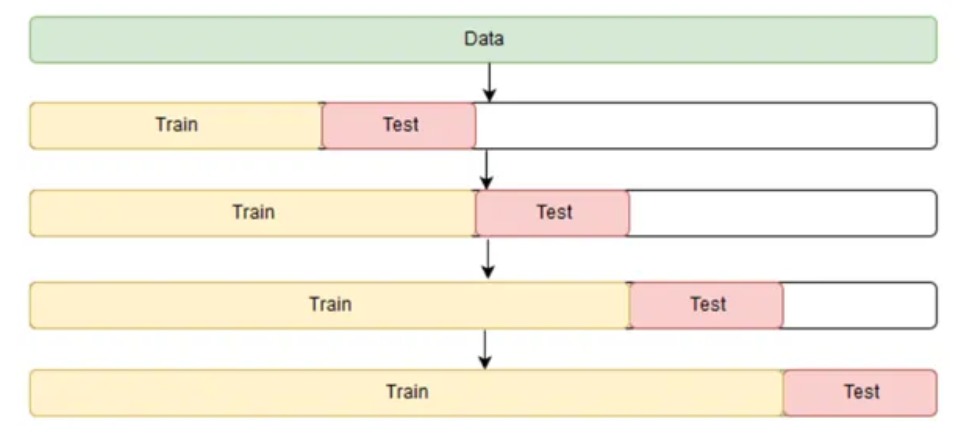
\includegraphics[width=0.65\linewidth]{images/rolling_cv.png}
  \caption{Cross-validation on a Rolling Basis (\cite{time_series_cv}).}
  \label{fig:rolling_cv}
\end{figure}

Figure~\ref{fig:rolling_cv} illustrates the basic idea of cross-validation on a rolling basis. The process starts with a small subset of the data used for training, with the subsequent subset used for testing. The data tested on is then used for the next training set and the subsequent subset is then used for testing. This procedure repeats until the end of the series.

Another approach is blocked cross-validation, where the series is divided into non-overlapping contiguous blocks, each block is used once as a validation set. This method avoids temporal leakage but may be less efficient in utilizing the full dataset compared to rolling schemes \cite{time_series_cv}.

Hyperparameter tuning for RNNs typically involve exploring architectural and training parameters. Important hyperparameter categories and examples include:

\begin{itemize}
    \item \textbf{Network Architecture}: Number of hidden layers, number of neurons per layer, choice of RNN variant.
    \item \textbf{Training Parameters}: Learning rate, optimizer type, batch size, sequence length, gradient clipping thresholds.
    \item \textbf{Regularization}: Dropout probability, weight decay.
\end{itemize}

Strategies such as grid search or random search using cross-validation can be used to explore the hyperparameter space and determine the best combination. The accuracy metric used to evaluate the models during the cross-validation process is entirely problem dependent, e.g. MSE used for regression, and accuracy for classification

\section{\textbf{Implementation}}

\subsection{\textbf{Technology Stack}}
All code was implemented in Python 3.12 using the following stack:
\begin{itemize}
    \item \textbf{Core Numerics}: \texttt{numpy}
    \item \textbf{Data Wrangling}: \texttt{pandas}
    \item \textbf{Time Series Utilities}: \texttt{statsmodels}
    \item \textbf{Visualization}: \texttt{matplotlib}
    \item \textbf{Preprocessing}: \texttt{scikit-learn}
    \item \textbf{Modeling}: \texttt{pytorch}
\end{itemize}

\subsection{\textbf{RNN Architectures}}
The RNNs investigated in this study were implemented using the PyTorch API. PyTorch is a highly customizable open-source deep learning framework. Each RNN type was defined as a custom \texttt{nn.Module} class, with a forward pass implementation tailored to the recurrence formula of the different architectures.
\begin{itemize}
    \item \textbf{ElmanRNN}: A tanh RNN cell (\texttt{nn.RNN}) followed by a linear output layer.
    \item \textbf{JordanRNN}: Forward pass implements the output-hidden state recurrence. The previous output is passed through an activation (\texttt{identity}/\texttt{sigmoid}/\texttt{softmax}/\texttt{tanh}) and then fed into the hidden layer at the current time step via a learned projection.
    \item \textbf{MultiRNN}: Implemented as a hybrid of the Elman and Jordan architectures, combining hidden-to-hidden and output-to-hidden recurrence.
\end{itemize}
All model implementations use the \texttt{tanh} hidden activation function and a final linear layer for regression outputs.
Implementations were also parameterized, which allows users to choose hidden layer size, output activation function, and output type (sequence-to-one vs. sequence-to-sequence). The implementations also included gradient clipping to prevent the exploding/vanishing gradient problem.

\subsection{\textbf{Training Utilities \& Pipeline}}
To keep code modular and compact, a set of utilities that encapsulates the steps in the model training pipeline were implemented:
\begin{itemize}
    \item \textbf{Sequence building}: \texttt{make\_sequences} converts $(X,y)$ into fixed-length windows and forecast horizon aligned targets with a configurable stride.
    \item \textbf{Datasets \& loaders}: \texttt{TimeSeriesDataset} wraps sequences as tensors. \texttt{DataLoaders} are created without shuffling (respecting temporal order) and without dropping tail batches.
    \item \textbf{Model factory}: \texttt{create\_model} constructs the requested model with the required architecture and parameters and moves it to the selected device (CPU/GPU).
    \item \textbf{Epoch routines}: \texttt{train\_one\_epoch} and \texttt{evaluate\_one\_epoch} standardize the train/validation passes, apply gradient clipping, and accumulate loss in a size-weighted manner across a single epoch.
    \item \textbf{Early stopping}: \texttt{fit\_early\_stopping} tracks the best validation loss, snapshots weights, and halts on \texttt{patience}. The best state dict is restored before evaluation.
    \item \textbf{Scaling helpers}: \texttt{fit\_seq\_scalers} and \texttt{transform\_seq} fit \texttt{MinMaxScalers} on the training data only and then transforms descriptive features and targets.
    \item \textbf{Prediction}: \texttt{predict\_all} performs batched inference.
\end{itemize}

\subsection{\textbf{Cross-Validation}}
The cross-validation process for hyperparameter tuning is handled by:
\begin{itemize}
    \item \textbf{Windowing}: \texttt{rolling\_windows} yields chronological (train, val) index slices with a user-defined train size, validation size, and step.
    \item \textbf{Hyperparameter config scoring}: \texttt{ts\_cv\_score} takes a model, fits scalers on each train slice, performs training with early stopping, inverse-transforms predictions, and returns per-fold scores and their summary stats.
    \item \textbf{Grid search}: \texttt{grid\_search\_ts\_cv} iterates over hyperparameter configuration grid for a given architecture, invokes \texttt{ts\_cv\_score}, and selects the configuration with minimal mean CV error.
\end{itemize}
This separation ensures no data is leaked from future time steps to past time steps.

\subsection{\textbf{Final Model Training}}
Final model training and evaluation logic is encapsulated in:
\begin{itemize}
    \item \textbf{fit\_best}: given the selected hyperparameter configuration, it carves a small tail for internal early stopping, fits scalers on the remaining training sequences, restores best weights, performs test inference, and inverse-transforms outputs.
    \item \textbf{Metrics}: pluggable metric functions (\texttt{RMSE}, \texttt{MAE}, \texttt{R2}) are passed as a dictionary, computed on original units, and returned alongside predictions for downstream plotting or tables.
    \item \textbf{Experiment driver}: \texttt{run\_experiments} loops over horizons and architectures, applies grid search + \texttt{fit\_best}, and collects results.
\end{itemize}

\section{\textbf{Empirical process}}

\subsection{\textbf{Objective}}
The objective of this study was to compare three simple recurrent neural network architectures, namely the Elman RNN, Jordan RNN and Multi-RNN, in the context of five different time series forecasting problems. Five real-world regression time series datasets were selected that represent a diverse range of temporal patterns, stationarity, and application domains.
The central aim of the study was to evaluate the relative strengths and weaknesses of the Elman, Jordan, and Multi-RNN architectures across different forecasting horizons, and to test whether the performance ranking of these models is consistent across various datasets or whether certain architectures are better suited to specific types of time series.
Feature standardization, sequence construction, training setup, and evaluation procedures ensure the empirical process was designed to isolate the effect of model architecture as the key property of interest under investigation.

\subsection{\textbf{Dataset Specific Preprocessing}}
\subsubsection{\textbf{AMD Stock Data}}
\begin{itemize}
    \item \texttt{Adj Close} was chosen as response, hence the redundant column \texttt{Close} was dropped.
    \item Rows with zero-valued opening prices were removed as these entries are most likely data entry errors, and there are only a few of them so removing them will not introduce any major bias into the dataset.
\end{itemize}

\subsubsection{\textbf{Air Quality}}
\begin{itemize}
    \item Several fields use the place holder value \textit{-200} to indicate sensor failures. These values were treated as missing entries.
    \item The dataset contains five sensor readings \texttt{PT08.S1(CO)}, \texttt{PT08.S2(NMHC)}, \texttt{PT08.S3(NOx)}, \texttt{PT08.S4(NO2)}, \texttt{PT08.S5(O3)}, and three meteorological variables \texttt{T}, \texttt{RH}, \texttt{AH}. It was found that the missing entries in these features were co-located. These rows were entirely removed from the dataset as they contained mostly missing values.
    \item Other missing values were interpolated using time-based interpolation, using the timestamp index to interpolate values between the nearest known points in time.
\end{itemize}

\subsubsection{\textbf{Garment Productivity}}
\begin{itemize}
    \item Invalid entries, such as entries missing key fields such as \texttt{date} or \texttt{actual\_productivity} (response) were removed.
    \item The \texttt{wip} column was entirely removed from the dataset, as it was missing half of its entries.
    \item The dataset contains a mix of numeric and categorical features. The categorical variables were converted into one-hot-encoded vectors using dummy encodings. This makes the categorical features usable in neural network based models.
\end{itemize}

\subsubsection{\textbf{Electric Production}}
No preprocessing needed to be done on the Electric Production dataset. It contains only a single feature measured over time.

\subsubsection{\textbf{Max Planck Institute Weather Data}}
No preprocessing was needed for this dataset, as it is a complete dataset containing no missing values or invalid entries.

\subsection{\textbf{Dataset Agnostic Preprocessing}}
\subsubsection{\textbf{Scaling}}
For all datasets, the descriptive and response features were normalized using scikit-learn's \texttt{MinMaxScaler}. During cross-validation and final model training, the scalers were fit on the training data only and then applied to the corresponding test and/or validation sets. This was done to prevent information from future time steps to leak into past time steps.
The \texttt{MinMaxScaler} was used because the RNN implementations use the tanh activation function, which outputs values in the range [-1, 1]. By scaling inputs and outputs into compatible ranges, the model training process was more stable, reducing the risk of vanishing or exploding gradients.

\subsubsection{\textbf{Sequence Construction}}
Each dataset was transformed into sequences of fixed length. This allowed the recurrent neural networks to receive a window of past observations as inputs and predict future values at specified horizons.
A sliding window procedure was used to construct the sequences. First the datasets were sorted by time stamp, and then for a given window length \texttt{L}, a contiguous block of \texttt{L} timesteps was extracted as an input sequence, and a value at a specified horizon was selected as the target. By moving the window forward one step at a time, multiple overlapping sequences were generated.
A moderate sequence length of 30 items was selected as this effectively balances temporal context while keeping compute costs manageable. The earlier items in longer sequences would be wastefully included, as their temporal information will be lost by overly extensive recurrence.
The study considered multiple horizons to evaluate the models' short-term and long-term predictive performance. Specifically predictions were made for horizons of 1, 3, 5, and 7 time steps ahead.
To clarify:
\begin{itemize}
    \item \textbf{Horizon = 1}: If the sequence length is 3 and the time series is \texttt{[1, 2, 3, 4, 5, 6, 7]}, then the input sequence is \texttt{[1, 2, 3]} and the target is \texttt{4}. This is simple next-item prediction.
    \item \textbf{Horizon = 3}. Under the same conditions, the input sequence would be \texttt{[1, 2, 3]} and the target is \texttt{6}
\end{itemize}
The models were trained in a sequence-to-one configuration, where each input sequence of 30 timesteps were used to predict a single output at the specified horizon. This allowed a fair comparison of Elman, Jordan, and Multi-RNN models across multiple datasets.

\subsection{\textbf{Model Training}}
After dataset preprocessing, the models were trained using a training setup that was designed to ensure stable learning, prevent overfitting, and allow for fair comparison of the three RNN model architectures across five different regression time series datasets.

\subsubsection{\textbf{Loss Function}}
All models were optimized using the Mean Squared Error loss function. This loss function is a common choice for regression problems, as it directly measures the squared deviation between predicted and true values, as well as being differentiable which is important for neural networks using gradient descent.

\subsubsection{\textbf{Optimization Algorithm}}
All models were trained using the Adam optimizer. The Adam optimizer (Adaptive Moment Estimation) is one of the most popular optimization algorithms used in training neural networks. It combines momentum, to smooth parameter updates by incorporating information from past gradients, and adaptive learning rate, to adjust step size of each parameter dynamically based on the history of gradients.

\subsubsection{\textbf{Regularization \& Stability Measures}}
To prevent overfitting and stabilize training, the following steps were taken:
\begin{itemize}
    \item \textbf{Weight Decay}: Incorporated in optimizer to penalize overly large weights and improve generalization.
    \item \textbf{Gradient Clipping}: A threshold was applied to the gradient during backpropagation, to clip the gradient and prevent instability during training.
    \item \textbf{Model Capacity Tuning}: Hidden layer size was included as a hyperparameter to be tuned during cross-validation, and sizes were varied to find the optimal hidden layer size for each model.
\end{itemize}

\subsubsection{\textbf{Early Stopping}}
Another measure taken to prevent overfitting was to use an early stopping mechanism when training the models. Training was halted when validation loss failed to improve after a fixed patience period (ranging from 8 to 12 epochs). At termination, the model parameters corresponding to the lowest validation loss were chosen as the optimal parameter set.

\subsubsection{\textbf{Batching and Data Loading}}
Input sequences were grouped into mini-batches using PyTorch's \texttt{DataLoader}. Batch sizes varied from 256 to 512 depending on the hyperparameter set being evaluated.

\subsubsection{\textbf{Hyperparameter Grid}}
A hyperparameter grid was used to tune the hyperparameters of each of the models during cross validation. The grid included the following parameters:
\begin{itemize}
    \item Hidden layer size: 32-256 units
    \item Learning rate: $1e-3$ to $5e-5$
    \item Batch size: 256 and 512
    \item Epochs: 60-120
    \item Patience for early stopping: 8-12
    \item Weight decay: $0$ to $1e-4$
\end{itemize}

\subsubsection{\textbf{Cross-Validation and Model Selection}}
Time series cross-validation was used to select optimal hyperparameters while respecting temporal order. After sequence construction the data was chronologically split (80/20) into a training portion and a test portion. The training portion was used to form rolling windows comprising of (train, validation) slices:
\begin{enumerate}
    \item For each window, \texttt{MinMaxScalers} were fit on the train slice only, and then applied to the validation slice to prevent look-ahead leakage.
    \item For each RNN architecture and hyperparameter configuration from the grid, a model was trained on the train slice and evaluated on the validation slice using RMSE computed on the original response scale.
    \item The cross-validation score for a model configuration was calculated as the mean RMSE across all rolling windows (folds).
\end{enumerate}
For each dataset, model and forecast horizon ([1, 3, 5, 7]), the hyperparameter configuration with the lowest mean CV RMSE was selected as the best hyperparameter configuration for that architecture. This process ensured a fair comparison driven only in difference between model architecture.

\subsubsection{\textbf{Final Model Training}}
Given the optimal hyperparameter set for a model architecture, forecast horizon, and dataset, final model training proceeded as follows:
\begin{enumerate}
    \item Within the entire training portion of the dataset, a small chronological tail (10\%) was reserved as a validation set to be used for early stopping.
    \item \texttt{MinMaxScalers} were then fit on the remaining training data.
    \item The model was then trained with MSE loss, and the Adam optimizer, using gradient clipping and weight decay where applicable.
\end{enumerate}

\subsection{\textbf{Final Model Evaluation}}
To provide an representative view of model accuracy and fit, three complementary metrics were calculated for each model on the test data set:
\begin{itemize}
    \item \textbf{RMSE}: Squared error.
    \item \textbf{MAE} Average absolute deviation.
    \item \boldmath{$R^2$} Explained variance.
\end{itemize}
Evaluating these metrics across the different models and forecast horizons reveal how the architectures perform compared to each other, and how they trade off short-term precision with long-range stability.

\subsection{\textbf{Reproducibility}}
To ensure reproducibility all random seeds were set consistently for NumPy and PyTorch. Nvidia CUDA deterministic flags were enabled where applicable.

\section{\textbf{Results \& discussion}}

\section{\textbf{Conclusion}}

\bibliographystyle{plain}
\bibliography{references}
\vspace{12pt}

\end{document}
